\chapter{System Architecture}
In this chapter, we present the system architecture for the proposed privacy-preserving location matching protocol. The main idea is to apply the principles of homomorphic encryption to location-based services, allowing clients to securely publish and performing queries using their positions without revealing sensitive information.

\section{Use Case}
To clearly understand the system operations, let's first analyze the use case of a client that wants to find the closest parking spot available. The client needs to compute the distances between its position and the parking spots, and finally decide whether to park or not and where.

Even through it seems a simple and straightforward mechanism, if we want to move the operations to the server, in order to preserve computational resources on the client side, a lot of challenges arise. The first one is to securely share the position of the client with the server, without exposing it to the workers. The second one is is not to leak sensible information about the clients, after the computation is finished.

In this scenario, it's not enough to simply encrypt the positions of the clients, as the workers need to compute the distances between the positions of the clients and the parking spots, that are also encrypted with a different key. To resolve this problem, we could just leave the parking position in clear text on the database, but this would expose the parking spots to the workers, that could then leak the information for profit. Thus, by selling the parking spots to third parties, they could are compromising the privacy of the system. In order to avoid this, and also achieve a full privacy-oriented protocol, we need to use a re-encryption mechanism, that allows the workers to compute the distances between the positions of the clients and the parking spots, without revealing the positions of the clients to the workers.

The distance problem is avoided by using the Z-order encoding, that allows us to reduce the problem of finding matching points into finding the maximum prefix of two bit strings. In our use case, the simulated server will perform a simple encrypted subtraction between the positions of the clients and the parking spots. At last, the only the client will be able to decrypt the result, which is a simple integer value that represents the distance between the two points (If the value is 0 is a perfect match). The client can then use this value to decide whether to park or not, and where. 

\section{System Overview}
The protocol is designed to combine a standard request-response protocol with a publish-subscribe mechanism.


\begin{figure}[h]
    \centering
    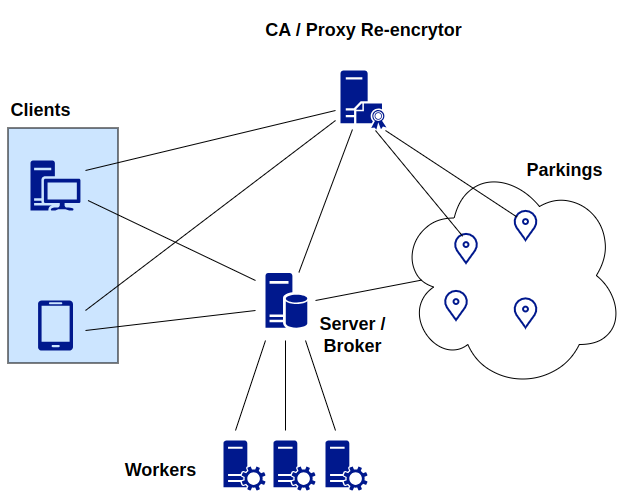
\includegraphics[width=8.5cm,height=5.5cm]{img/architecture-scheme.png}
    \caption{Visualization of the system architecture for the proposed privacy-preserving location matching protocol.}
    \label{fig:architecture}
\end{figure}

Homomorphic encryption incurs high computational costs, so the system optimizes performance by splitting the workload: the server handles only essential data processing, while workers compute the distances between client positions. Since HE allows computations on encrypted data, this approach preserves the privacy of clients' locations without compromising efficiency.

\section{Actors}

\subsection{Location Data Source}
The Location Data Source (LDS), commonly referred to as sensors or parkings, are responsible for collecting and publishing location data. In our system, we assume they independently publish their data to the broker, based on the event they register. For instance, if a sensor detects a free parking spot, it publishes the information to the broker, that will start the encryption protocol. This happens also when a parking spot is occupied, allowing the system to keep track of the available parking spots in real-time.

Note that by maintaining the availability of the parking spots, independent from the clients, we can ensure that the system is able to provide privacy-preserving updates to the server. Conversely, if the clients were also responsible for reserving the parking spots, they would need to expose their positions to the server, which would compromise the privacy of the system.

\subsection{Mobile Clients}
MCs or Mobile Clients are the users of the system. Their main interest is to receive updates on the closest available parking spots, based on their current position. 

In our system, the client's responsibilities are very limited, as they do not trust the server and all the other actors involved in the protocol. They only need to publish their encrypted position to the server, wait for the computation to finish, and then receive the results.

\subsection{Server}
The Backend Server (commonly called Information Broker) is the central component of the system, responsible for managing the communication between clients and sensors. It also acts like a database, handling and storing the encrypted parking spots data.

This centralized component is crucial in the architecture, as it allows all sort of mobile actors (including clients and LDs) to have a persistent connection with the system, although it's not enough if we want to achieve a full zero-trust protocol.

Thanks to HE, the server can perform computation without knowing the clear text positions of the other actors.

\subsection{Certification Authority / Proxy}
The certification authority (CA) is a trusted entity responsible for storing the public keys of the clients and managing the public/private keys of the parking spots. Because he is a trusted entity, the CA knows the private keys of the parking spots. Thus, it can generate the symmetric translation keys required for a secure computation of the client distances without revealing clear text positions.

In our system, the CA also acts like a proxy re-encryptor\cite{POLYAKOV2017FastPRE}, as it is responsible for managing the right keys for the homomorphic operation made on the encrypted data. 

\subsection{Worker}
The name Worker refers to a generic computational unit of the system, that can handle tasks from the server rewarded with a digital currency. In our case, the workers are responsible for computing the distances between the positions of the clients and the parking spots, using the homomorphic encryption scheme. 

The workers' digital reward can be described as a token that allows them to request tasks from the server. In this way, each client can act as a worker, contributing to the overall computation of the system.

\section{Network Protocol and Communication}
\subsection{Usage of different network protocols}

The MQTT protocol is used for the communication between the clients and the server. It is necessary to use a pub/sub mechanism in order to keep alive the connection between the two entities. This is achieved by having the client subscribe to a topic, while the proxy publishes updates to that topic.

Moreover, the server is responsible for managing the connection with the LDs, allowing the clients to receive updates on the parking spots. In this way, the client $MC_i$ \textbf{publishes} its position $Area_j$ to the topic $ID_{MC_i}$. The server can then apply the homomorphic operations on the data, using the keys provided by the CA.

When the computation is finished, the broker publishes the results to the topic $ID_{MC_i}$, allowing the client to receive the updates on the parking spots. The client can then \textbf{subscribe} to the topic $ID_{MC_i}$ to receive updates on the parking spots.

The HTTP protocol is used for the communication between the CA and the other entities of the system. Because the CA performs atomic actions, such as key generation and translation, it is necessary to use a request-response protocol to ensure that the operations are performed in a secure and reliable way.

%\newpage

\section{Protocol Overview}
The system is designed to allow the following operations:

\begin{table}[h]
\renewcommand{\arraystretch}{1.3}
\small
\begin{tabularx}{\linewidth}{|l|X|X|X|p{4cm}|}
\hline
\textbf{API} & \textbf{Subject} & \textbf{Protocol} & \textbf{Receiver} & \textbf{Payload} \\ \hline

Position Encoding Parameters & Clients / LDs & HTTP GET & Server & - \\ \hline

Key Obtain & LDs & HTTP GET & CA / Proxy & $\{id: ID_{park_j}\}$ \\ \hline

Key Share & Client & HTTP POST & CA / Proxy & $\{id: ID_{mc},\ \text{pub. key: } k_{mc}^+\}$ \\ \hline

Position Publish & Client & MQTT PUB & Server & $\{position: \xi_{mc}(P_i)\}$ \\ \hline

Topic Subscription & Client & MQTT SUB & Server & $\{topics: [position, distance]\}$ \\ \hline

Location Publish & LDs & HTTP POST & Server & $\{\xi_{park_j}(P_j),\ id: ID_{park_j},\ \text{status} \in \{\text{free}, \text{occ.}\}\}$ \\ \hline

Translate Locations & Server & HTTP GET & CA / Proxy & $\{positions: [\xi_{park_j}(P_{j})]\}$ \\ \hline

Work Request & Worker & HTTP GET & Server & - \\ \hline

Task Finished & Worker & HTTP POST & Server & $\{worker: w_i,\ task: t_j,\ result: \xi_{park_j \to mc_i}(R)\}$ \\ \hline

Distance Publish & Server & MQTT PUB & Client & $\{distances: [\forall j \in P,\ \xi_{mc_i}(R)]\}$ \\ \hline

\end{tabularx}
\caption{System Operations Aligned with Architecture}
\label{table:system-operations}
\end{table}

\section{Distance Preference}

As we mentioned in the Table \ref{table:system-operations}, the first operation that both the MCs and LDs need to perform is to obtain the position encoding parameters from the server. In this section, we will analyze why this is necessary and how it works.

The necessity of translating a GPS reference into a grid position encoding comes with some limitations. First of all, the grid-like structure requires a fixed size for both the whole area and the single grid cell. This operation is performed by the server, in order to ensure consistency across the whole system. This operation could be performed also by the single actors, but only if they are aware of a standardized measurement unit. Moreover, the subscribers could be interested in creating a custom grid, like system some orders of magnitude larger then the others, that should still maintain the original atomic cell size.

For our study case, we will assume that the centralized server is responsible for managing the parameters. In this way, he can generate a grid that contains the geographical area of Bologna, Italy, where the simulated parking spots are located.

% \newpage
\section{Scenario}


\begin{figure}[h]
    \centering
    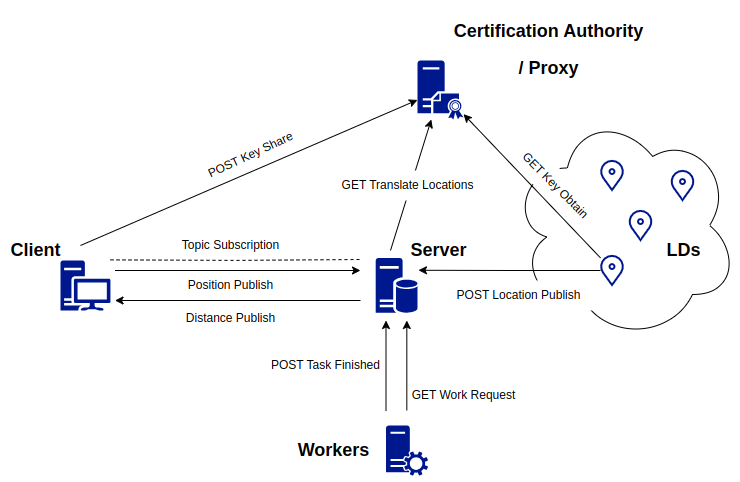
\includegraphics[width=12cm,height=7.5cm]{img/workflow.png}
    \caption{Visualization of the protocol flow}
    \label{fig:protocol-flow}
\end{figure}

\subsection{Protocol Flow}

We can summarize the protocol flow in the following steps as shown in \cref{fig:protocol-flow}:

\begin{enumerate}
    \item The clients and the parking spots register to the system, after that they receive the general position encoding parameter from the server using the \textbf{Position Encoding Parameters} API via HTTP GET request. The parameters are used to encode the positions of the clients and the parking spots. \emph{(API: \texttt{Position Encoding Parameters}, Payload: \{none\} $\to \{encoding\_params: [\text{z-order}, \text{precision}, \text{working area}, \text{grid cell size}]\}$})
    \item The mobile client $MC_i$ generates a new public/private key pair $(k_{mc_i}^+, k_{mc_i}^-)$ and sends the public key to the certification authority (CA) using the \textbf{Key Share} API via an HTTP POST request. \emph{(API: \texttt{Key Share}, Payload: $\{id: ID_{mc_i},\ k_{mc_i}^+\} \to { \text{None} }$)}
    \item After the CA verifies the client, it generates a symmetric key $k_{mc_i, park_j}$ for each parking spot $park_j$. The operation of key generation is performed by \emph{Key Translation}$(pp, k_{mc_i}^+, k_{park_j}^-)$, where $pp$ is the public parameters of the system, $k_{mc_i}^+$ is the public key of the client, and $k_{park_j}^-$ is the private key of the parking spot. Note that the translation operation must be done each time a new parking spot is added to the system.
    \item The $MC_i$ establish a MQTT connection with the server and subscribes to the topic $ID_{MC_i}$, which is used to receive updates on the parking spots. This is done using the \textbf{Topic Subscription} API via MQTT. \emph{(API: \texttt{Topic Subscription}, Payload: $\{topics: [position, distance]\}$)}
    \item The client will then send the encrypted position $\xi_{mc}(P_i)$ to the server, where $P_i$ is the encoded position of the client. The encryption is done using the public key $k_{mc_i}^+$, ensuring that only the client can decrypt the position. This is done using the \textbf{Position Publish} API via MQTT. \emph{(API: \texttt{Position Publish}, Payload: $\{position: \xi_{mc}(P_i)\}$)}
    \item The server receives the location and start the translation process, by invoking the \textbf{Translate Locations} API via HTTP GET request to the CA. The CA then re-encrypts the position for each parking spot using the associated key $k_{park_j \to mc_i}$, creating the re-encrypted blob $[\forall j \in \text{P},\ \xi_{mc_i}(P_j)]$. \emph{(API: \texttt{Translate Locations}, Payload: $\{positions: [\xi_{park_j}(P_j)]\}$)}
    \item The server will then spread the re-encrypted positions to the workers, by invoking the \textbf{Work Request} API via HTTP GET request. The workers will then compute the distances between the client position and the parking spots, using the re-encrypted positions. \emph{(API: \texttt{Work Request}, $Payload: \{ worker: w_i \} \to \{task: t_j \} $})
    \item Once the workers compute the distances (or other metrics) between client and parking spots, they send the result back using the \textbf{Task Finished} API via HTTP POST request. The result is a re-encrypted blob containing the distances between the client position and the parking spots. \emph{(API: \texttt{Task Finished}, Payload: $\{worker: w_i,\ task: t_j,\ result: \xi_{park_j \to mc_i}(R)\}$)}
    \item The server then publishes the aggregated results to the client via MQTT using the \textbf{Distance Publish} API. The payload contains the distances between the client position and the parking spots, re-encrypted with the client's public key. \emph{(API: \texttt{Distance Publish}, Payload: $\{distances: [\forall j \in P,\ \xi_{mc_i}(R)]\}$)}
    \item Finally, the client receives the re-encrypted results, decrypts them using its private key $k_{mc_i}^-$, checks weather the location satisfies the area matching condition.
\end{enumerate}

\section{Security Considerations}

The main goal of the study is to provide a privacy-preserving location-matching protocol, that allows clients to securely publish and query their positions without revealing sensitive information. In order to fulfill this goal, we need to ensure that the system is attack-resistant and that the privacy of the clients is preserved.

In the earlier approach \cite{genova2024helamqtt}, the position-matching protocol used Euclidean distance calculations between client locations and parking spots provided by a trusted CA. While the server could not directly access this data, the mechanism inadvertently exposed the positions of mobile clients (MCs). The vulnerability stemmed from the lack of client authentication, enabling malicious actors to impersonate legitimate clients and intercept traffic. An attacker could exploit this by conducting a binary search on the client’s location, sending iterative queries based on subscribed topics. By progressively refining the search area, the attacker could pinpoint the client’s exact position, violating location privacy.

This showcased that HE is secure if and only if the encryption and decryption operation are performed correctly, preferably by the client itself.

As we also mentioned in the previous attack, the system is vulnerable to a lack of authentication of the clients. Moreover, if an attacker was able to read the network traffic, he could also manipulate the communication in order to interfere with the pub/sub mechanism.

In my own implementation, I addressed those issues by introducing different techniques from the state of the art, such as using a proxy re-encryptor and a position encoding mechanism based on Z-order. The choice of leaving the decryption operation to the client ensures that no one is able to read the sensitive data, despite an increase of computational resources required to re-encrypt each position for each parking spot.

\subsection{Threat Model} \label{subsec:threatmodel}

In this section, we will analyze the threat model of the system, identifying the potential attackers and their capabilities. 


\subsection{Mitigation Strategies Malicious Actors}

\begin{table}[h]
\renewcommand{\arraystretch}{1.3}
\small
\begin{tabularx}{\linewidth}{|l|X|X|}
\hline
\textbf{Adversary} & \textbf{Goal / Attack} & \textbf{Mitigation Strategy} \\ \hline

Malicious Client &
Impersonate another client or send fake position updates. &
Use digital signatures: at the time of authentication with the CA the client signs a digital contract that ensures that he is the one trying to access the system. \\ \hline

Malicious Worker &
Manipulate computation results or leak client-sensitive data. &
Because the user has no way of finding out if an information has been manipulated during homomorphic phase, the server need to implement a mechanism of \emph{fake workload} to test workers reliability. \\ \hline

Malicious Server &
Access or manipulate sensitive client data or computational outcomes. &
Because the server could only drop the communication or modify packets, but not leak sensitive informations. It's suggested to have multiple backup servers independent one from the other. \\ \hline

Network Attacker &
Intercept and read client-sensitive data from network traffic. &
All the traffic is HE encrypted. \\ \hline

\end{tabularx}
\caption{Adversarial Threats and Mitigation Strategies}
\label{table:adversaries}
\end{table}

In the \cref{table:adversaries}, we summarize the potential adversaries and their goals, along with the mitigation strategies that can be employed to counteract their attacks. It's also important to notice that one of the assumptions of the system was that the CA is a trusted entity, moreover if an attacker is able to compromise the CA, he can also compromise the whole system. Thus, it's not worth to consider the CA as an adversary.
